\section{Линейная регрессионная модель}

Мы начнем с классической модели линейной регрессии, или линейной модели, восходящей к Лежандру и Гауссу в начале 19 века. Набор данных $\textbf{x}$ для модели линейной регрессии состоит из $n$ точек $\textbf{x}_1, \textbf{x}_2, \ldots, \textbf{x}_n$, где каждый $\textbf{x}_i$ сам по себе является парой, скажем
\begin{equation}
	\textbf{x}_i = (\textbf{c}_i, y_i).
\end{equation}
Здесь $\textbf{c}_i$ --- это $1 \times p$ вектор $\textbf{c}_i = (c_{il}, c_{i2}, \ldots, c_{ip})$, называемый \textit{вектором признаков} или \textit{предиктором}, а $y_i$ --- действительное число, называемое \textit{ответом}.

Пусть $\mu_i$ указывает условное ожидание $i$-го ответа $y_i$ с учетом предиктора $\textbf{c}_i$,
\begin{equation}
	\mu_i = \text{E}(y_i|\textbf{c}_i) \quad (i = 1,2, \ldots, n).
\end{equation}
Ключевое предположение в линейной модели состоит в том, что $\mu_i$ представляет собой линейную комбинацию компонентов предиктора $\textbf{c}_i$,
\begin{equation}
	\mu_i = \textbf{c}_i \bm{\beta} = \sum\limits_{j=1}^{p} c_{ij} \beta_j.
\end{equation}
\textit{Вектор параметров}, или \textit{параметр регрессии}, $\bm{\beta} = (\beta_1, \beta_2, \ldots, \beta_p)^\text{T}$ неизвестен, обычная цель регрессионного анализа состоит в том, чтобы вывести $\bm{\beta}$ из наблюдаемых данных $\textbf{x} = (\textbf{x}_1, \textbf{x}_2, \ldots, \textbf{x}_n)$. В квадратичной регрессии (7.20) для данных холостирамина ответ $y_i$ --- это улучшение для $i$-го человека, признак $\textbf{c}_i$ --- это вектор $(1, z_i, z_i^2)$ и $\bm{\beta} = (\beta_0, \beta_1, \beta_2)^\text{T}$. \underline{Примечание}: «Линейность» в линейной регрессии относится к линейной форме математического ожидания (9.3). Нет никакого противоречия в том, что линейная модель (7.20) является квадратичной функцией $z$.

Вероятностная структура линейной модели обычно выражается как
\begin{equation}
	y_i = \textbf{c}_i \bm{\beta} + \varepsilon_i \quad \text{для} \quad i = 1,2,\ldots,n.
\end{equation}
Предполагается, что ошибка $\varepsilon_i$ в (9.4) является случайной выборкой из неизвестного \textit{распределения ошибок} $F$ с математическим ожиданием $0$,
\begin{equation}
	F \to (\varepsilon_1, \varepsilon_2, \ldots, \varepsilon_n) = \bm{\varepsilon} \quad [\text{E}_F(\bm{\varepsilon})=0].
\end{equation}

Заметим, что (9.4), (9.5) влекут
\begin{align}
	\text{E}(y_i|\textbf{c}_i) & = \text{E}(\textbf{c}_i \bm{\beta}+\varepsilon_i|\textbf{c}_i) = \text{E}(\textbf{c}_i \bm{\beta}|\textbf{c}_i) + \text{E}(\varepsilon_i|\textbf{c}_i) \notag \\
	& = \textbf{c}_i \bm{\beta},
\end{align}
что является предположением о линейности (9.3). Здесь мы использовали тот факт, что математическое ожидание $\text{E}(\varepsilon_i|\textbf{c}_i)$ совпадает с безусловным ожиданием $\text{E}(\varepsilon_i) = 0$, поскольку $\varepsilon_i$ выбираются независимо от $\textbf{c}_i$.

Мы хотим оценить вектор коэффициентов $\bm{\beta}$ из наблюдаемых данных $(\textbf{c}_1, y_1), (\textbf{c}_2, y_2), \ldots, (\textbf{c}_n, y_n)$. Пробное значение $\bm{\beta}$, скажем $\textbf{b}$, дает \textit{остаточную квадратичную ошибку}
\begin{equation}
	\text{RSE}(\textbf{b}) = \sum\limits_{i=1}^{n} (y_i - \textbf{c}_i \textbf{b})^2,
\end{equation}
как в уравнении (7.21). Оценка \textit{методом наименьших квадратов} $\bm{\beta}$ --- это значение $\hat{\bm{\beta}}$ из $\textbf{b}$, которое минимизирует $\text{RSE}(\textbf{b})$,
\begin{equation}
	\text{RSE}(\hat{\bm{\beta}}) = \min_{\textbf{b}} [\text{RSE(\textbf{b})}].
\end{equation}
Пусть $\textbf{C}$ --- матрица размерности $n \times p$ с $i$-й строкой $\textbf{c}_i$, а \textbf{y} --- вектор $(y_1, y_2, \ldots, y_n)^\text{T}$. Тогда оценка методом наименьших квадратов является решением следующего уравнения
\begin{equation}
	\textbf{C}^\text{T} \textbf{C} \hat{\bm{\beta}} = \textbf{C}^\text{T} \textbf{y}
\end{equation}

\noindent
\noindent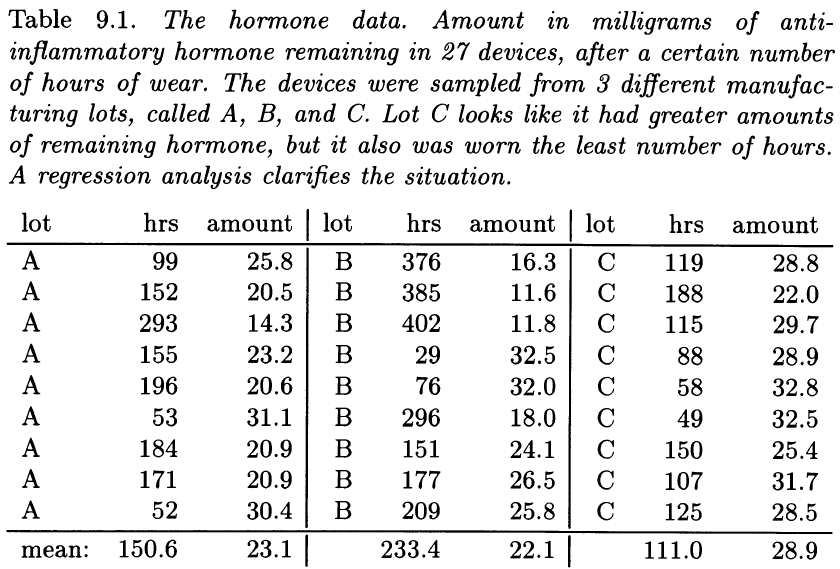
\includegraphics[width=\linewidth]{9/t91}
\newline
и задается формулой
\begin{equation}
	\hat{\bm{\beta}} = (\textbf{C}^\text{T} \textbf{C})^{-1} \textbf{C}^\text{T} \textbf{y}.
\end{equation}